\subsubsection{Spectator Prediction Class Diagram}

\begin{figure}[H]
    \centering
    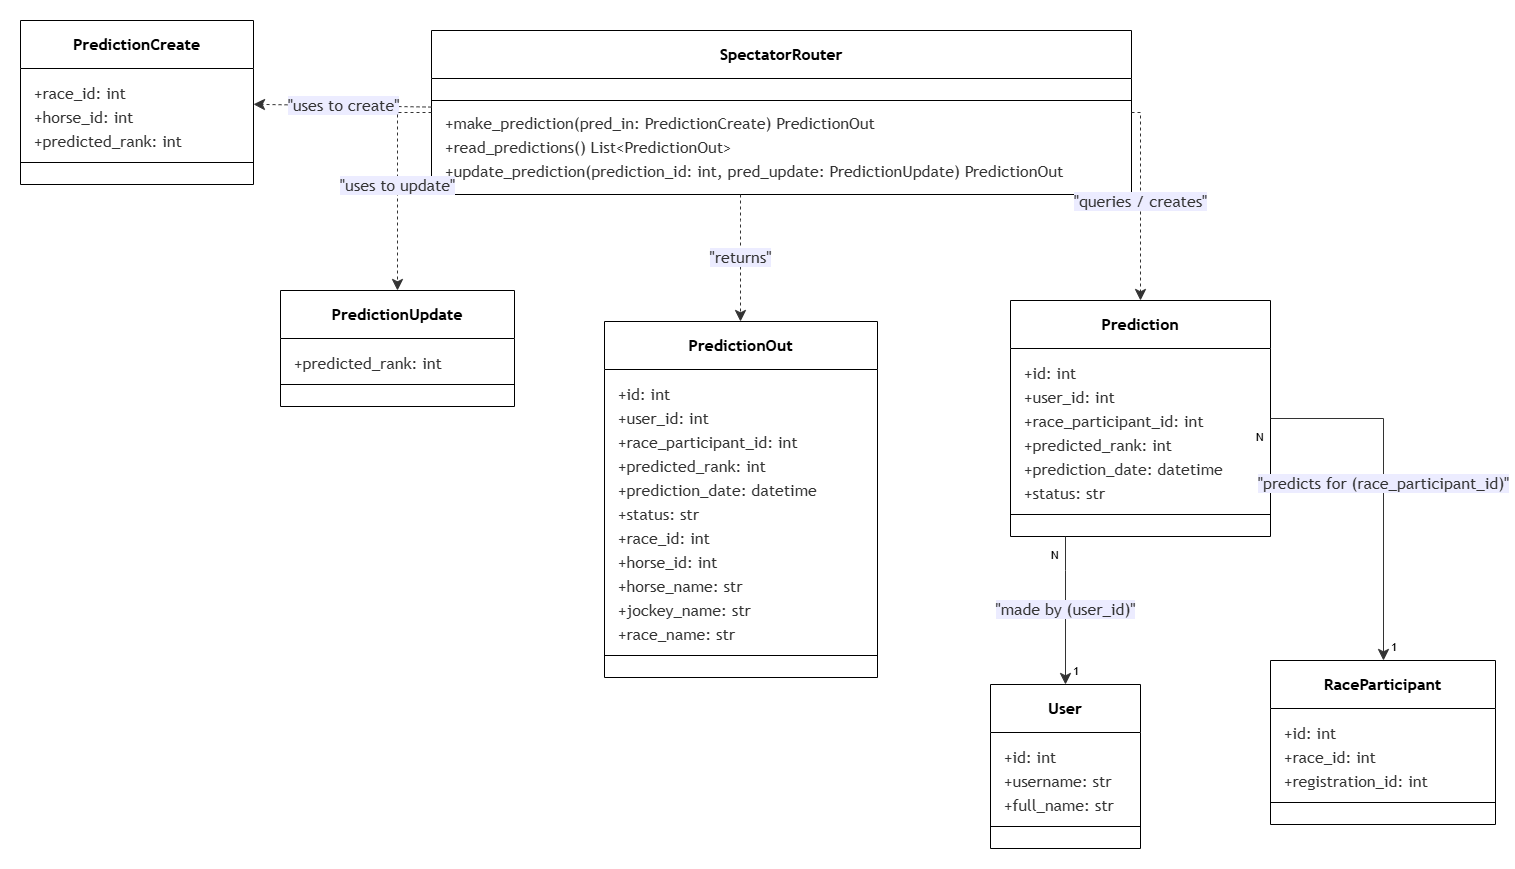
\includegraphics[width=\textwidth]{figures/design/spectator/prediction_class_diagram.png}
    \caption{Spectator Prediction Class Diagram}
    \label{fig:spectator_prediction_class_diagram}
\end{figure}


\subsubsection{Class Specification}

\begingroup
\small
\setlength{\tabcolsep}{3pt}
\TableStart{|>{\raggedright\arraybackslash}p{0.15\textwidth}|>{\raggedright\arraybackslash}p{0.31\textwidth}|>{\raggedright\arraybackslash}p{0.14\textwidth}|>{\raggedright\arraybackslash}p{0.25\textwidth}|}
\textbf{Class} & \textbf{Attributes / Methods} & \textbf{Type} & \textbf{Description} \\
\hline
SpectatorRouter & make\_prediction(), read\_predictions(), update\_prediction() & controller / route & Handles HTTP requests related to spectator predictions (create, read, update). \\
\hline
PredictionCreate & race\_id, horse\_id, predicted\_rank & DTO & Input data transfer object used to create a new prediction. \\
\hline
PredictionUpdate & predicted\_rank & DTO & Input data transfer object used to update the predicted rank. \\
\hline
PredictionOut & id, user\_id, race\_participant\_id, predicted\_rank, prediction\_date, status, race\_id, horse\_id, horse\_name, jockey\_name, race\_name & DTO & Output data transfer object containing detailed prediction details and related information. \\
\hline
Prediction & id, user\_id, race\_participant\_id, predicted\_rank, prediction\_date, status & entity & Database entity that stores the user's prediction information. \\
\hline
User & id, username, full\_name & entity & Database entity representing an application user who makes predictions. \\
\hline
RaceParticipant & id, race\_id, registration\_id & entity & Database entity representing a participant in a race being predicted. \\
\TableFinish{Spectator Prediction class specification}{tab:spectator_prediction_class_spec}
\endgroup

\subsubsection{Spectator Personal Profile Class Diagram}

\begin{figure}[H]
    \centering
    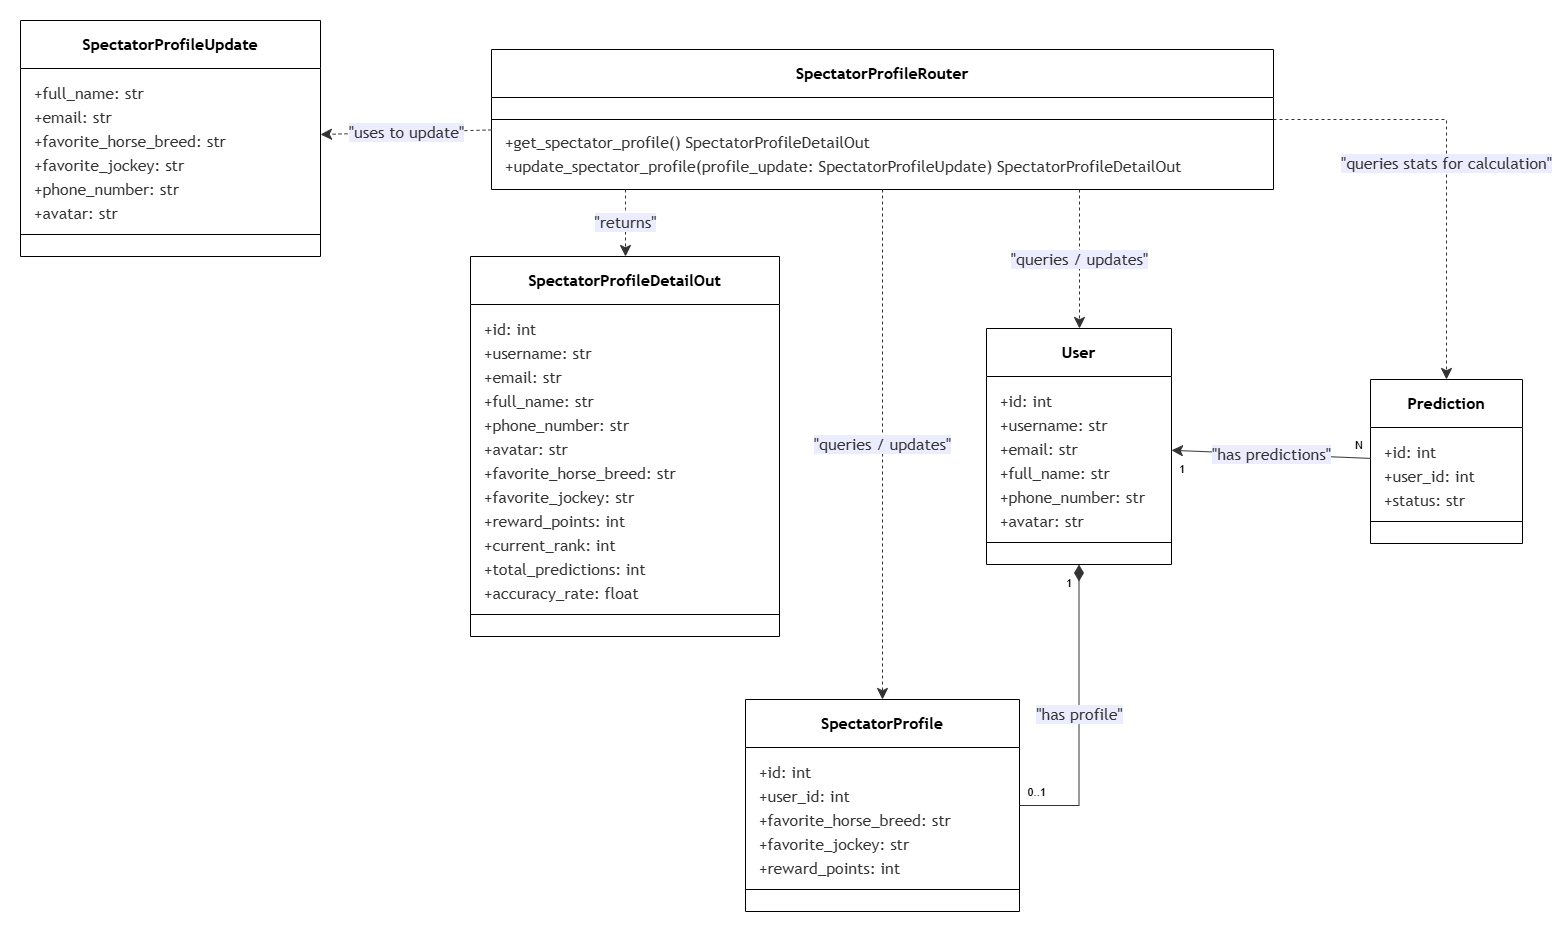
\includegraphics[width=\textwidth]{figures/design/spectator/personal_profile_class_diagram.png}
    \caption{Spectator Personal Profile Class Diagram}
    \label{fig:spectator_personal_profile_class_diagram}
\end{figure}


\subsubsection{Class Specification}

\begingroup
\small
\setlength{\tabcolsep}{3pt}
\TableStart{|>{\raggedright\arraybackslash}p{0.18\textwidth}|>{\raggedright\arraybackslash}p{0.28\textwidth}|>{\raggedright\arraybackslash}p{0.14\textwidth}|>{\raggedright\arraybackslash}p{0.25\textwidth}|}
\textbf{Class} & \textbf{Attributes / Methods} & \textbf{Type} & \textbf{Description} \\
\hline
SpectatorProfileRouter & get\_spectator\_profile(), update\_spectator\_profile() & controller / route & Handles HTTP requests related to spectator profiles, including retrieving profile details and updating information. \\
\hline
SpectatorProfileUpdate & full\_name, email, favorite\_horse\_breed, favorite\_jockey, phone\_number, avatar & DTO & Input data transfer object containing the fields that a spectator can update in their profile. \\
\hline
SpectatorProfileDetailOut & id, username, email, full\_name, phone\_number, avatar, favorite\_horse\_breed, favorite\_jockey, reward\_points, current\_rank, total\_predictions, accuracy\_rate & DTO & Output data transfer object returning the comprehensive profile information, including calculated statistical metrics. \\
\hline
User & id, username, email, full\_name, phone\_number, avatar & entity & Database entity representing the core authentication account information of the user. \\
\hline
SpectatorProfile & id, user\_id, favorite\_horse\_breed, favorite\_jockey, reward\_points & entity & Database entity storing additional profile information specific to the spectator role. \\
\hline
Prediction & id, user\_id, status & entity & Database entity referenced to aggregate user prediction counts and statistics for profile calculation. \\
\TableFinish{Spectator Profile class specification}{tab:spectator_profile_class_spec}
\endgroup


\subsubsection{Schedule and Result Class Diagram}
\begin{figure}[H]
    \centering
    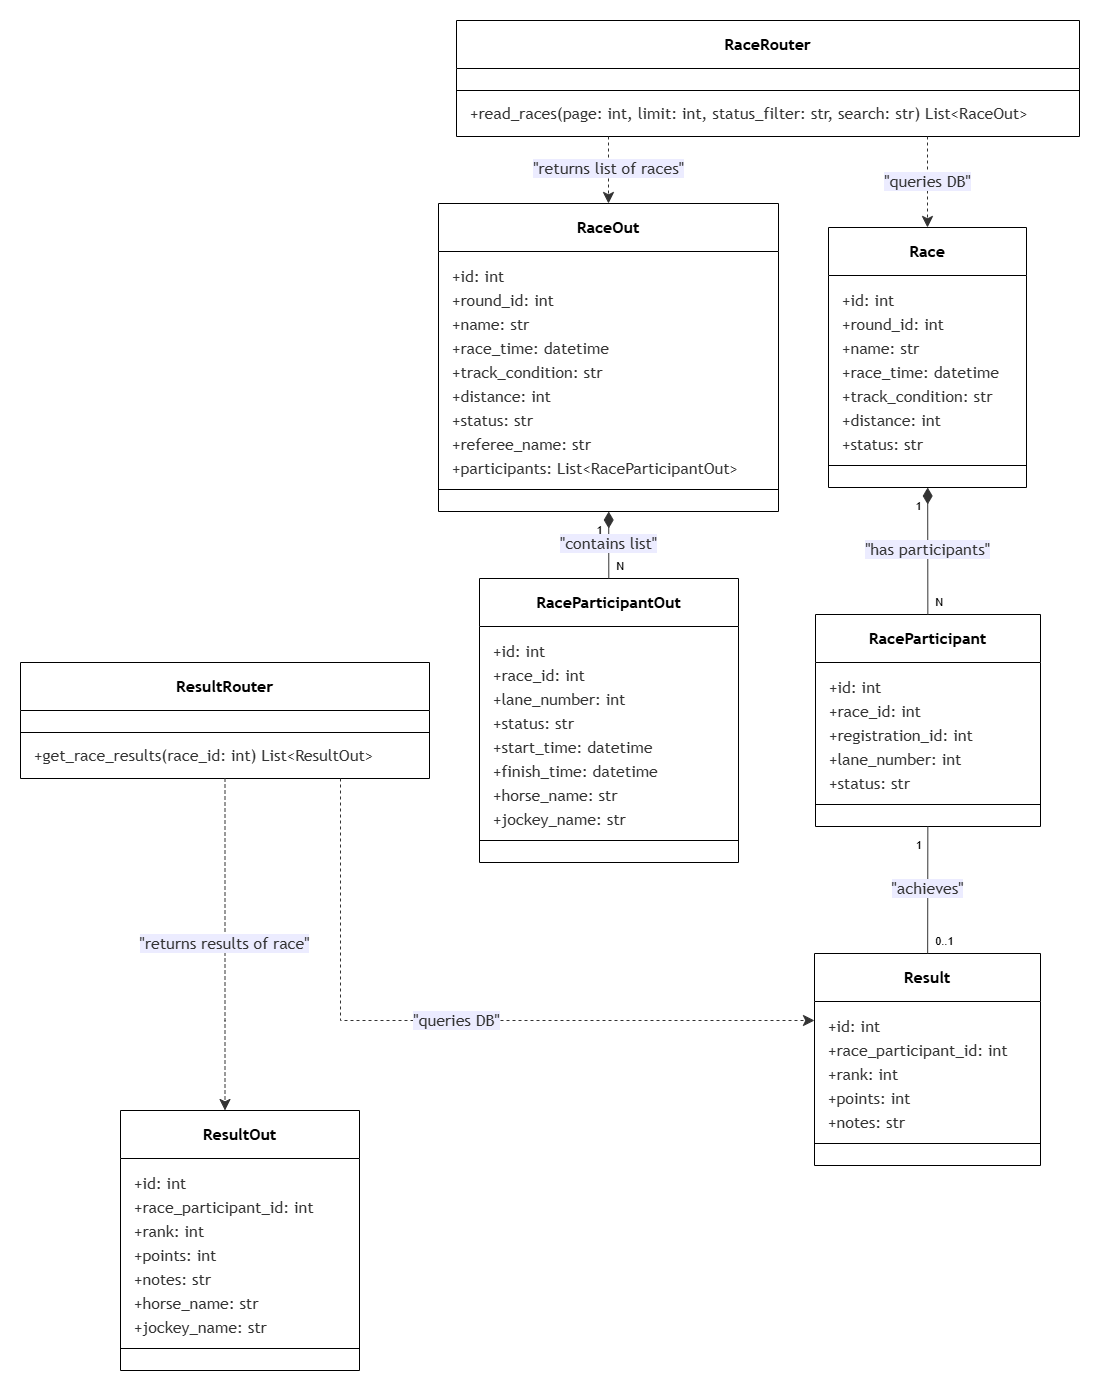
\includegraphics[width=\textwidth]{figures/design/spectator/schedule_and_results_class_diagram.png}
    \caption{Schedule and Result Class Diagram}
    \label{fig:schedule_and_result_class_diagram}
\end{figure}

\subsubsection{Class Specification}

\begingroup
\small
\setlength{\tabcolsep}{3pt}
\TableStart{|>{\raggedright\arraybackslash}p{0.18\textwidth}|>{\raggedright\arraybackslash}p{0.28\textwidth}|>{\raggedright\arraybackslash}p{0.14\textwidth}|>{\raggedright\arraybackslash}p{0.25\textwidth}|}
\textbf{Class} & \textbf{Attributes / Methods} & \textbf{Type} & \textbf{Description} \\
\hline
ScheduleRouter & read\_schedules() & controller / route & Handles HTTP requests to retrieve and filter the list of scheduled horse races. \\
\hline
ResultRouter & get\_race\_results() & controller / route & Handles HTTP requests to retrieve the official results of a specific race. \\
\hline
RaceOut & id, round\_id, name, race\_time, track\_condition, distance, status, referee\_name, participants & DTO & Output data transfer object containing comprehensive race details and its participants. \\
\hline
RaceParticipantOut & id, race\_id, lane\_number, status, start\_time, finish\_time, horse\_name, jockey\_name & DTO & Output data transfer object representing detailed information of a participant within a race. \\
\hline
ResultOut & id, race\_participant\_id, rank, points, notes, horse\_name, jockey\_name & DTO & Output data transfer object returning the final standings and details of a race result. \\
\hline
Race & id, round\_id, name, race\_time, track\_condition, distance, status & entity & Database entity storing core information of a horse racing event. \\
\hline
RaceParticipant & id, race\_id, registration\_id, lane\_number, status & entity & Database entity representing a registered horse and jockey combination participating in a race. \\
\hline
Result & id, race\_participant\_id, rank, points, notes & entity & Database entity storing the official placement and points scored by a race participant. \\
\TableFinish{Schedule and Result class specification}{tab:schedule_and_result_class_spec}
\endgroup

\subsubsection{Horse and Jockey Rankings Class Diagram}
\begin{figure}[H]
    \centering
    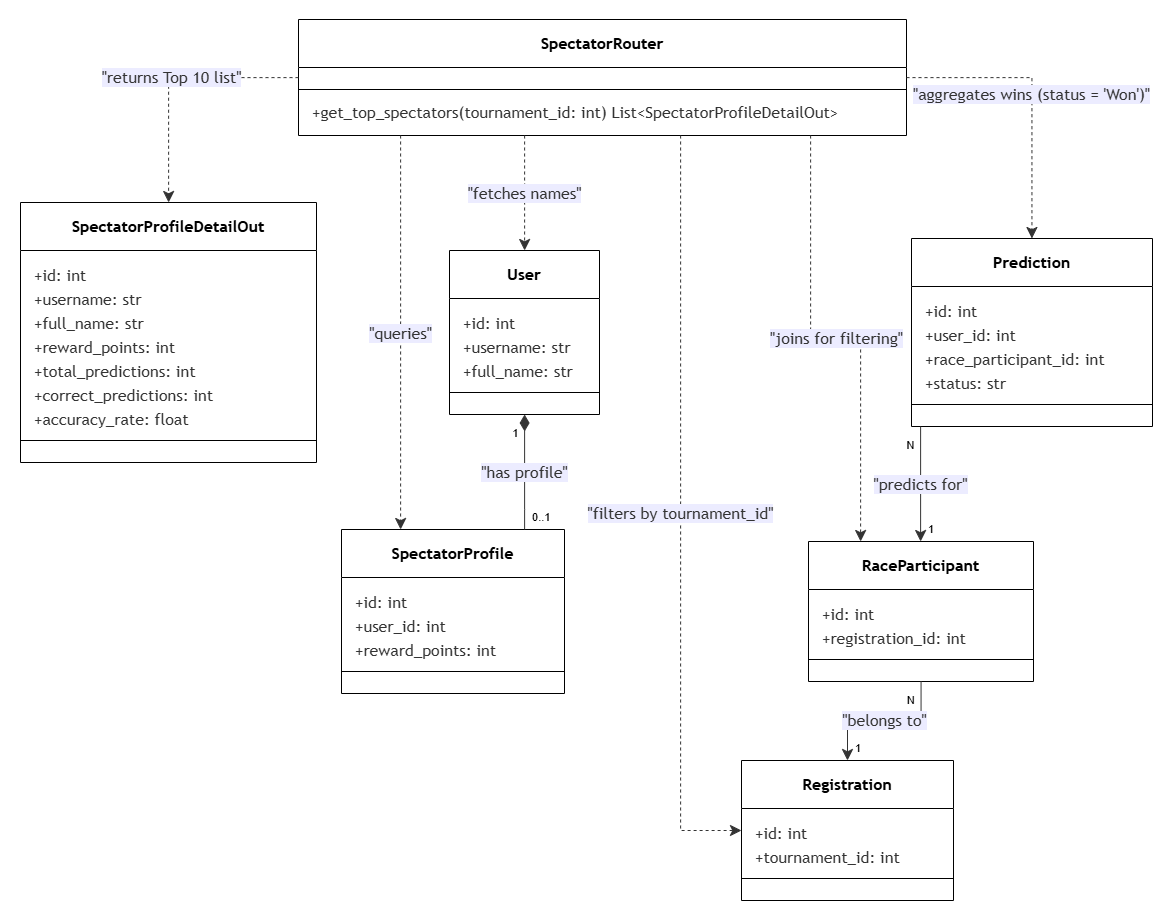
\includegraphics[width=\textwidth]{figures/design/spectator/horse_and_jockey_leaderboard_class_dg.png}
    \caption{Horse and Jockey Rankings Class Diagram}
    \label{fig:horse_jockey_rankings_class_diagram}
\end{figure}

\subsubsection{Class Specification}

\begingroup
\small
\setlength{\tabcolsep}{3pt}
\TableStart{|>{\raggedright\arraybackslash}p{0.18\textwidth}|>{\raggedright\arraybackslash}p{0.28\textwidth}|>{\raggedright\arraybackslash}p{0.14\textwidth}|>{\raggedright\arraybackslash}p{0.25\textwidth}|}
\textbf{Class} & \textbf{Attributes / Methods} & \textbf{Type} & \textbf{Description} \\
\hline
ResultRouter & read\_rankings() & controller / route & Handles HTTP requests to retrieve leaderboard rankings filtered by tournament. \\
\hline
RankingOut & id, entity\_type, entity\_id, entity\_name, points, rank, updated\_at & DTO & Output data transfer object returning the formatted ranking list of horses or jockeys. \\
\hline
Ranking & id, tournament\_id, entity\_type, entity\_id, points, rank & entity & Database entity that stores the computed scores and standings within a tournament. \\
\hline
Horse & id, name & entity & Database entity representing horse information used when the ranking entity type is a horse. \\
\hline
JockeyProfile & id, user\_id & entity & Database entity representing jockey profiles used when the ranking entity type is a jockey. \\
\hline
User & id, full\_name & entity & Database entity representing core user accounts, used to fetch the full name of jockeys. \\
\TableFinish{Horse and Jockey Rankings class specification}{tab:horse_jockey_rankings_class_spec}
\endgroup

\subsubsection{Top Spectators Leaderboard Class Diagram}
\begin{figure}[H]
    \centering
    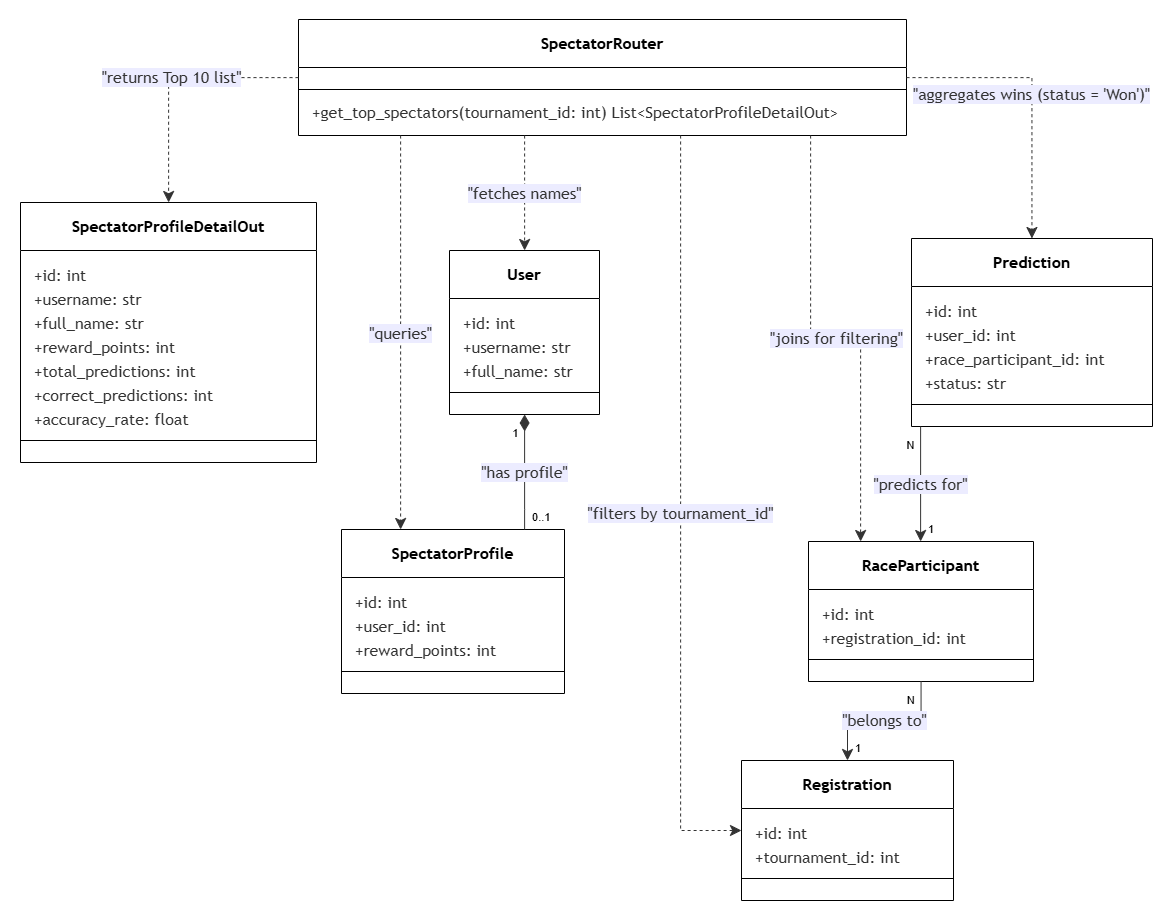
\includegraphics[width=\textwidth]{figures/design/spectator/top10_spectators_leaderboard_class_dg.png}
    \caption{Top 10 Spectators Leaderboard Class Diagram}
    \label{fig:top_spectators_class_diagram}
\end{figure}

\subsubsection{Class Specification}

\begingroup
\small
\setlength{\tabcolsep}{3pt}
\TableStart{|>{\raggedright\arraybackslash}p{0.18\textwidth}|>{\raggedright\arraybackslash}p{0.28\textwidth}|>{\raggedright\arraybackslash}p{0.14\textwidth}|>{\raggedright\arraybackslash}p{0.25\textwidth}|}
\textbf{Class} & \textbf{Attributes / Methods} & \textbf{Type} & \textbf{Description} \\
\hline
SpectatorRouter & get\_top\_spectators() & controller / route & Handles HTTP requests to aggregate and retrieve the leaderboard of top 10 spectators filtered by tournament. \\
\hline
SpectatorProfileDetailOut & id, username, full\_name, reward\_points, total\_predictions, correct\_predictions, accuracy\_rate & DTO & Output data transfer object returning the top spectator profiles along with their performance metrics. \\
\hline
User & id, username, full\_name & entity & Database entity representing the user accounts to fetch the profile identity names. \\
\hline
SpectatorProfile & id, user\_id, reward\_points & entity & Database entity storing spectator-specific statistics and total reward points. \\
\hline
Prediction & id, user\_id, race\_participant\_id, status & entity & Database entity used to aggregate and calculate accurate prediction statistics (where status is 'Won'). \\
\hline
RaceParticipant & id, registration\_id & entity & Database entity representing race participants, utilized to join and filter predictions by race context. \\
\hline
Registration & id, tournament\_id & entity & Database entity representing tournament registrations, used to filter leaderboard data by specific tournament. \\
\TableFinish{Top Spectators Leaderboard class specification}{tab:top_spectators_class_spec}
\endgroup